\begin{figure}[htbp]
  \centering
  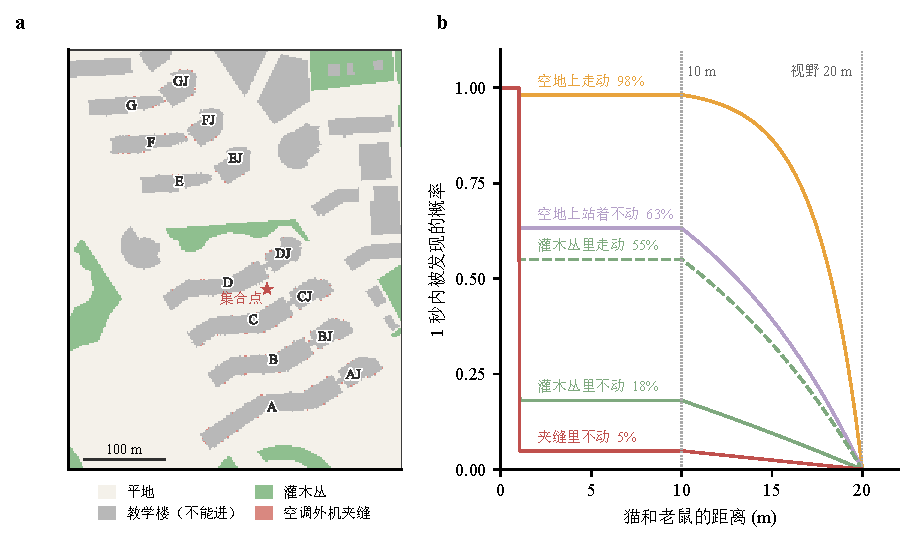
\includegraphics[width=\textwidth]{fig0_environment.pdf}
  \caption{\figlead{场地取自 OpenStreetMap 的 A–G 楼一带，“藏在哪里、动不动”决定了被发现的快慢。}
  \textbf{a}，栅格化后的场地（0.5 m 一格）。红点是沿外墙放置的空调外机夹缝（合成）；红星是开局集合点，位于 C、D、CJ、DJ 四栋楼之间。
  \textbf{b}，一只猫在不同距离上看着老鼠时，老鼠 1 秒内被发现的概率。曲线旁的百分比是 5 m 处的数值。10 m 以内速率不变，之后线性下降，到 20 m 降为 0；1 m 以内必定被发现。}
  \label{fig:env}
\end{figure}

\subsection{博弈建模：被抓即转化的部分可观测随机博弈}
本文把一轮游戏写成一个 30 名玩家、有限时域的部分可观测随机博弈（POSG）
\begin{equation*}
\mathcal{G}=\langle \mathcal{N}, \mathcal{S}, \rho_0, \{\mathcal{A}_i\}, \{\mathcal{O}_i\}, O, P, \{r_i\}, T\rangle .
\end{equation*}
玩家集合 $\mathcal{N}$ 为 30 人。状态 $s_t$ 包括所有人的位置、速度、体力、身份（猫或老鼠），夜跑路人的位置和目的地，以及每只猫对每只老鼠“是否正在盯住”的标记。初始分布 $\rho_0$ 是：10 只猫、20 只老鼠在集合点附近随机出生。观测函数 $O$ 把全局状态映射为每个人的观测 $o_i\in\mathcal{O}_i$，由第~\ref{sec:detect} 节的发现模型定义：每个人只看得到自己的状态和视线内、20 m 以内的人，具体构成见表~\ref{tab:obs}。时域 $T$ 为 30 分钟（3600 步，步长 $\Delta t=0.5$ s），老鼠全部被抓时这一局提前结束。

状态转移中最特别的是身份转移：老鼠 $i$ 与猫 $j$ 的距离小于 0.6 m 即被抓，$i$ 的身份立刻变为猫，同时记 $j$ 抓到一只。因此玩家总数不变，但两个阵营的人数随时间变化，一名玩家在一轮中可能先当老鼠、后当猫。本文把这两个阶段分开处理：老鼠阶段的目标是活得久，猫阶段的目标是多抓。开局猫原地数 60 秒。运动方面，冲刺 4 m/s、慢跑 2.5 m/s、走 1.5 m/s，灌木丛和夹缝里最快 0.8 m/s；冲刺最多持续 20 s，走路或站着时恢复。碰撞检测把每步分成 4 个子步，撞墙后沿墙滑动。

这是一个一般和博弈：老鼠的存活收益和猫的抓捕收益加起来并不是常数，双方收益也不互为相反数。老鼠之间没有直接冲突，但任何一只老鼠被抓，都会让其余老鼠面对的猫多一只。

\subsection{发现模型与反事实对照}
\label{sec:detect}
猫 $j$ 能“看到”老鼠 $i$ 的前提是两人之间视线不被楼挡住，且距离 $d<R=20$ m（晚上路灯下的视野）。在这个前提下，每一步以概率 $1-e^{-\lambda\Delta t}$ 发现对方，速率为
\begin{equation}
\lambda = \lambda_0 \cdot g(d) \cdot f_{\text{静}}^{\,\mathbb{1}[\text{静止}]} \cdot f_{\text{地形}}, \qquad
g(d)=\min\!\left(1,\ 2\left(1-\tfrac{d}{R}\right)\right)_{+},
\end{equation}
其中 $\lambda_0=4\ \text{s}^{-1}$。速度低于 0.3 m/s 视为静止，$f_{\text{静}}=0.25$；在灌木丛里 $f_{\text{地形}}=0.2$，在夹缝里 $f_{\text{地形}}=0.05$，在平地上为 1。1 m 以内必定发现。一旦被发现，猫会一直盯住目标，直到视线被楼挡住或距离超过 20 m。图~\ref{fig:env}b 给出了各状态下 1 秒内被发现的概率：在 5 m 处，空地上走动是 98\%，夹缝里不动只有 5\%。老鼠这一侧，6 个夜跑路人在路上慢跑，老鼠在 5 m 以外认不出路人是不是猫，所以远处的路人和猫一样会引发逃跑。

这些系数是笔者根据游戏体验设定的，不是测量值。现实中，藏在夹缝里、站着不动当然更难被发现；本文并不怀疑这一点。实验中把某个系数改成 1（即“这个因素不再带来隐蔽优势”），是一种\textbf{反事实对照}：如果改掉某个因素之后，躲的优势就消失了，就说明在这个模型里，躲的优势正是由这个因素带来的；如果改掉之后优势还在，说明还有别的原因（例如藏身点的位置、路线）。这样做的目的是找出“躲为什么有效”，而不是判断现实中藏身处是否更隐蔽。本文分别做三组对照：只取消静止的优势（$f_{\text{静}}=1$）、只取消地形的优势（$f_{\text{灌木}}=f_{\text{夹缝}}=1$）、以及两者都取消。

\subsection{脚本策略}
\label{sec:script}
脚本策略是写好固定规则的猫和老鼠，用来回答 RQ1–RQ3，也作为强化学习的对照。猫的策略分三层：看见老鼠，就按对方速度预判 2 s 后的位置并去拦截；跟丢了，就去最后看见的位置附近搜 30 秒；都没有，就巡逻——全队共享一张 20 m × 20 m 的“多久没人搜过”表，每只猫从 4 个随机候选格中挑最久没搜过的一个去搜。

老鼠有五种策略。\textbf{跑}：慢跑游走，一见到猫（或 5 m 外认不出的路人）就冲刺逃离，逃跑方向从 16 个方向里选，既要远离威胁，又要保证前方 1.5 m 和 3 m 都能走。\textbf{躲}：走到最近的灌木或夹缝藏好不动，猫进入 10 m 才逃，逃完再换一个藏身点，选点时兼顾“离自己近、离威胁远”。\textbf{只躲灌木}和\textbf{只躲夹缝}与之相同，但只选一种藏身点。\textbf{原地不动}：不找掩体，就地站着，猫进入 10 m 才逃。

\subsection{上下两轮之间的策略转化}
\label{sec:imitate}
为回答 RQ3，本文让 20 只老鼠中躲的比例 $x$ 分别取 0、0.25、0.5、0.75、1（其余都跑），每个 $x$ 跑 256 局，得到躲者和跑者各自的收益（30 分钟内的平均存活时间）$\pi_H(x)$ 和 $\pi_R(x)$。在此基础上模拟第一轮结束后的模仿：每只老鼠随机看同一局里的一个同伴，若同伴采用另一种策略，就以概率
\begin{equation}
p = \frac{1}{1+\exp\!\big(-(\pi_{\text{同伴}}-\pi_{\text{自己}})/K\big)}
\end{equation}
改用同伴的策略\cite{szabo1998,traulsen2006}。$K$ 表示“看别人结果时的随机性”：$K$ 越小，越只跟着收益高的人学。$\pi$ 用的是这一局里两人各自的实际存活时间，所以即使躲的平均收益更高，也会有“这一局躲的人运气差、跑的人运气好”的情况，从而出现从躲到跑的反方向转化。本文统计两个方向的转化比例，以及第二轮躲的比例。

\subsection{双方共同训练的 PPO}
\label{sec:obs}
猫和老鼠各用一张网络（两层、每层 256 个单元），同一阵营的所有个体共用参数。老鼠被抓后，下一步起改由猫网络控制。两张网络同时用 PPO 训练，互为对方的环境。两张网络的输入相同，共 218 维（表~\ref{tab:obs}）。

\begin{table}[htbp]
  \centering\small
  \caption{强化学习的观测（每人 218 维）}
  \label{tab:obs}
  \renewcommand{\arraystretch}{1.2}
  \begin{tabularx}{\textwidth}{@{}lcX@{}}
    \toprule
    内容 & 维数 & 说明\\
    \midrule
    自身状态 & 11 & 位置、速度、剩余体力、已用时间、脚下地形、场上猫的比例、自己的身份（被抓后所有人都知道，属于公开信息）\\
    8 个方向到墙的距离 & 8 & 20 m 以内\\
    周围地形 & 147 & 以自己为中心 14 m × 14 m 的 7 × 7 局部图，灌木、夹缝、建筑三个通道\\
    最近 5 个对手 & 25 & 相对位置、速度、是否有效。老鼠：自己看见的猫和认不出的路人（用路人的真实速度）；猫：自己或 30 m 内队友正在盯住的老鼠（相当于喊话报位置）\\
    最近 4 个队友 & 20 & 只包括视线内、20 m 以内的队友\\
    记忆 & 3 & 最后一次看见对手的位置和距今时间\\
    提示 & 4 & 当前藏身目标、巡逻目标的方向\\
    \bottomrule
  \end{tabularx}
\end{table}

老鼠有 27 个动作：停下，8 个方向 × 3 档速度，外加“沿路去最近的藏身点”和“冲刺逃离”两个现成动作。猫有 20 个动作：停下，8 个方向 × 2 档速度，外加“沿路追（带预判）”“去最后看见的地方”“巡逻”三个现成动作。本文没有给猫“包抄”动作，围捕只能通过方向动作和追击动作的配合出现。

老鼠每活一步得 $\Delta t/60$，即每活 1 分钟得 1 分；被抓后，它作为老鼠的轨迹终止。猫的奖励分两组：\textbf{个人奖励}组自己抓到一只得 1 分，是真实游戏“抓得最多的猫有奖”的近似（真实游戏是按名次发奖，这里改成按只计分）；\textbf{团队奖励}组全队每抓到一只，抓捕前已经是猫的每个成员平分 1 分。为了检验“团队奖励的问题出在功劳被稀释”这个猜想，又加了两组：\textbf{混合奖励}取个人奖励和团队奖励各一半；\textbf{按参与分配}把每次抓捕的 1 分只分给抓捕瞬间离受害者 15 m 以内、抓捕前已经是猫的成员（平均每次约 3.4 只）。后者是一种局部共享奖励：它仍然奖励“在场”而不是精确地衡量每只猫的贡献，并不是严格意义上的差分奖励。“按参与分配”和团队奖励相比改了两件事：分到功劳的猫变少了（奖励更集中），而且分到的是在场的猫（奖励与行为挂钩）。为了把这两点分开，再加一组\textbf{随机分配}对照：每次抓捕分给几只猫与“按参与分配”完全相同，但这几只猫是从全体猫中随机抽的，与它在不在场无关（实测只有约四成恰好在场）。

共同训练还有一个已知问题：双方只和对方的\textbf{当前}版本对局，容易学成只能打败这一个对手的对策。为此本文加了\textbf{历史对手池}组（一种基于历史快照的自我对弈）：每 25 轮把双方网络存一份快照；每开一批新局，每方从快照里随机抽 4 份，分给不同的局。一半的局让当前老鼠对历史猫，只训练老鼠；另一半让历史老鼠对当前猫，只训练猫。这样每方实际用到的样本只有普通组的一半，所以历史对手池组训练 600 轮，样本量与普通组的 300 轮大致相同。为了把“对手更多样”和“样本减半、训练轮数加倍”这两个因素分开，另设\textbf{只用最新对手}组：流程完全相同，但快照池只保留最近一份。

抓捕判定在每个移动子步都检查一次距离（一步 0.5 秒分 4 个子步），避免猫和老鼠迎面跑过、在两次检查之间擦身而过却不算抓到。各方的动作只改写自己的状态，例如猫的巡逻动作不会改动老鼠的目标点。

计算优势时，GAE 需要知道下一步还是不是同一张网络在控制这个人。本文为每个人、每一步记录角色掩码 $m_{t+1}$：老鼠在 $t\to t+1$ 之间被抓，则 $m_{t+1}=0$，这一段对老鼠网络而言就是终止；某一局老鼠全部被抓后，这一局也立即终止，不再产生训练样本。记 $d_t$ 为这一步是否终止，则
\begin{equation}
\delta_t = r_t + \gamma\, m_{t+1}\,(1-d_t)\, V(o_{t+1}) - V(o_t),\qquad
\hat A_t = \delta_t + \gamma\lambda\, m_{t+1}\,(1-d_t)\,\hat A_{t+1}.
\end{equation}
训练要最小化的损失是剪切形式的 PPO 目标，加上价值损失和熵正则：
\begin{equation}
\begin{aligned}
L(\theta)={}&-\mathbb{E}_t\!\left[\min\!\big(\rho_t\hat A_t,\ \operatorname{clip}(\rho_t,1-\epsilon,1+\epsilon)\hat A_t\big)\right]\\
&+\tfrac12\,\mathbb{E}_t\!\left[(V_\theta(o_t)-\hat R_t)^2\right]-c_H\,\mathbb{E}_t\!\left[\mathcal H(\pi_\theta(\cdot|o_t))\right],
\end{aligned}
\end{equation}
其中 $\rho_t=\pi_\theta(a_t|o_t)/\pi_{\theta_{\text{old}}}(a_t|o_t)$，价值目标 $\hat R_t=\hat A_t+V_{\theta_{\text{old}}}(o_t)$。超参数见表~\ref{tab:hp}。折扣 $\gamma=0.995$ 对应的“半衰期”约 69 秒，也就是说，网络更看重一两分钟内的生存，对几分钟以后的收益看得较轻。

\begin{table}[htbp]
  \centering\small
  \caption{训练超参数}
  \label{tab:hp}
  \begin{tabular}{@{}ll@{\qquad}ll@{}}
    \toprule
    参数 & 取值 & 参数 & 取值\\
    \midrule
    并行局数 & 64 & 每轮采样步数 & 128 步（64 s）\\
    一局时长 & 30 分钟（3600 步） & 训练轮数 & 300（对手池两组 600）\\
    折扣 $\gamma$ / GAE $\lambda$ & 0.995 / 0.95 & 剪切 $\epsilon$ & 0.2\\
    学习率（Adam） & $3\times10^{-4}$ & 每轮更新 & 4 遍，小批量 16384\\
    熵系数 $c_H$ & 0.01 & 梯度裁剪 & 0.5\\
    训练组 & 8 组（见正文） & 每组训练种子 & 3 个\\
    \bottomrule
  \end{tabular}
\end{table}

\subsection{评价指标}
存活时间指一轮 30 分钟内的平均存活时间，没被抓的老鼠记 30 分钟。同一局里的老鼠面对同一批猫，彼此并不独立，所以本文的置信区间一律\textbf{按局}重采样（2000 次自举，取 95\% 区间）\cite{agarwal2021}；比较两种策略时，用同一局内的配对差。强化学习的结果先按训练种子分别评估（每个种子 64 局，评估用与训练不同的固定随机种子），组均值取各种子均值的平均；置信区间用分层自举，先重抽训练种子，再在种子内重抽局，这样区间同时反映对局的随机性和训练种子之间的差异。只有 3 个种子时，这个区间很宽，也不够精确，所以强化学习部分的比较只作探索性结论。老鼠行为用五类时间占比描述：静止、在灌木丛里、在夹缝里、贴楼 2 m 以内、冲刺，这五类可以重叠，加起来不必是 100\%。

围捕指标在每次抓捕的瞬间计算，只统计抓捕之前就已经是猫的个体：一是受害者 15 m 内有没有至少 2 只猫；二是包围度 $1-\theta_{\max}/2\pi$，其中 $\theta_{\max}$ 是 20 m 内的猫相对受害者的最大角度空缺，猫全在同一侧时接近 0，四面包围时接近 1。这两个量描述的是抓捕瞬间猫的空间聚集，并不直接等于合作，因为场上猫越多，它们自然越容易聚在一起。猫之间的分配用开局 10 只猫的抓捕数基尼系数描述。基尼系数衡量分配的不均匀程度：0 表示每只猫抓到的数量完全相同，越接近 1 表示抓捕越集中在少数几只猫身上。
